\chapter{Evaluation}
\label{cha:evaluation}
\vspace{0.4 cm} 

In this chapter, the proposed system is validated and the results are evaluated.
Starting by describing how the system is tested at home to assess the feasibility of the proposed method. Subsequently, where and how the system is tested for experimental validation. Finally, an evaluation of the achieved results is presented. The data collector implemented on a Raspberry Pi has been placed in a place of social interest. In this place of social interest, I manually collected the ground truth for training and evaluating the model. The Mosquitto MQTT Broker, the MongoDB database and the Back-End part for receiving and storing the data in the database have been executed on the U-Hopper server. The final Back-End part for analyzing the data has been executed on my computer to adapt the parameters and train the Machine Learning model. After this chapter, it will be clear how the system has been validated and what the results achieved by the proposed system are. Overall conclusions are discussed in the next chapter.


\section{Experimental validation}
\label{sec:expval}
\vspace{0.2 cm} 

Due to the complex situation of this period due to COVID-19 and the limitations imposed on people, it was necessary to test the functioning of the system at home and verify the feasibility of the first part of the proposed method, i.e. detect the devices in the area. The tests were conducted on different days with the aim of revealing how many devices are in a determinate room of the house. As can be seen from figure~\ref{fig:sniffertest}, $\sim$ 66.000 Wi-Fi probe request frames are collected and the values of RSSI of the detected devices are divided into two main ranges. A value of RSSI in range -35 $\div$ -69 indicates that the device is close to the data collector, i.e. in the kitchen. Instead, a value of RSSI in range -69 $\div$ -91 indicates that the device is away from the data collector, i.e. not in the kitchen. Random encounters that do not belong to the house are rare and there are randomized MACs related to devices that are not connected to the home Wi-Fi network.

\begin{figure}[h]
\centering 
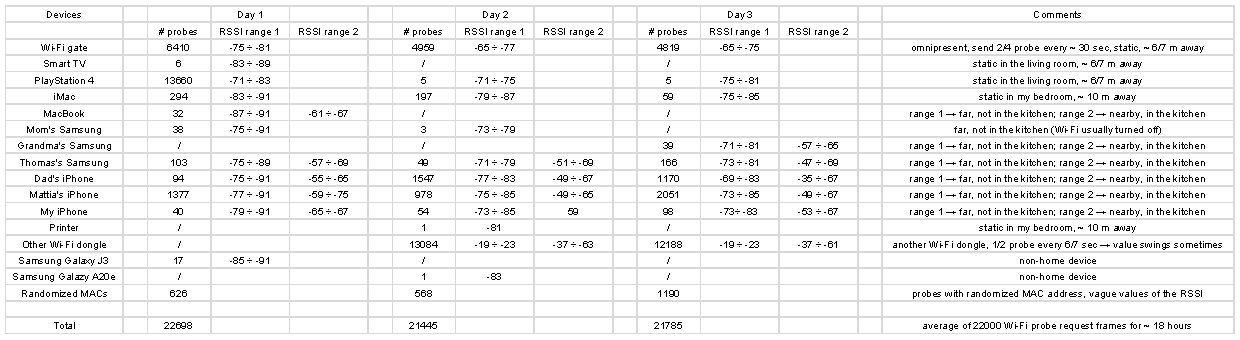
\includegraphics[width=1\textwidth]{images/sniffertest} 
\caption{Presentation of home test results.}
\label{fig:sniffertest}
\end{figure}

Subsequently, with the reduction of restrictions on personal mobility, it was possible to conduct an experimental validation and a data collection in a place of social interest with moderate mobility. The case study is to estimate the customers present in a Cafe, whose owner allowed me to conduct the experimentation in this delicate moment.

The data collector implemented on a Raspberry Pi model 2B has been placed in this Cafe and connected to an electrical source. In this place of social interest, I manually collected the ground truth with a random look strategy on my computer for training and evaluating the model.

The Mosquitto MQTT Broker, the MongoDB database and the Back-End part for receiving and storing the data in the database have been executed on the U-Hopper server.

Experimental environment considerations: Wi-Fi dongle (with a range of $\sim$ 10 meters) can cover all the Cafe area and detect all the devices of the people. The Cafe does not have a Wi-Fi network but, when I go there to collect the ground truth, it uses the hotspot from my phone to send data to the server.

The final part of the Back-End for data analysis was executed on my computer to adapt the parameters of the cleaning part for the case study. After cleaning the data and obtaining the presence of devices, it is possible to prepare and train the Machine Learning model with the collected ground truth and the number of devices revealed in the timestamps when the ground truth was collected.

% In the end, we store the results in the database instead of sending them to a hypothetical consumer of this type of system.

The management of the different time processes is shown in figure~\ref{fig:timeprocesses}:
\begin{itemize}
  \item Probe revelations from the data collector: a random point process with different MAC addresses.
  \item Presence of devices: a cadlag step function based on the revelations of the MAC addresses, obtained after the cleaning of the collected data.
  \item Collection of the ground truth: a sampling of the number people present, a random point process asynchronous with respect to the probe revealed and devices revealed.
\end{itemize}

\begin{figure}[h]
\centering 
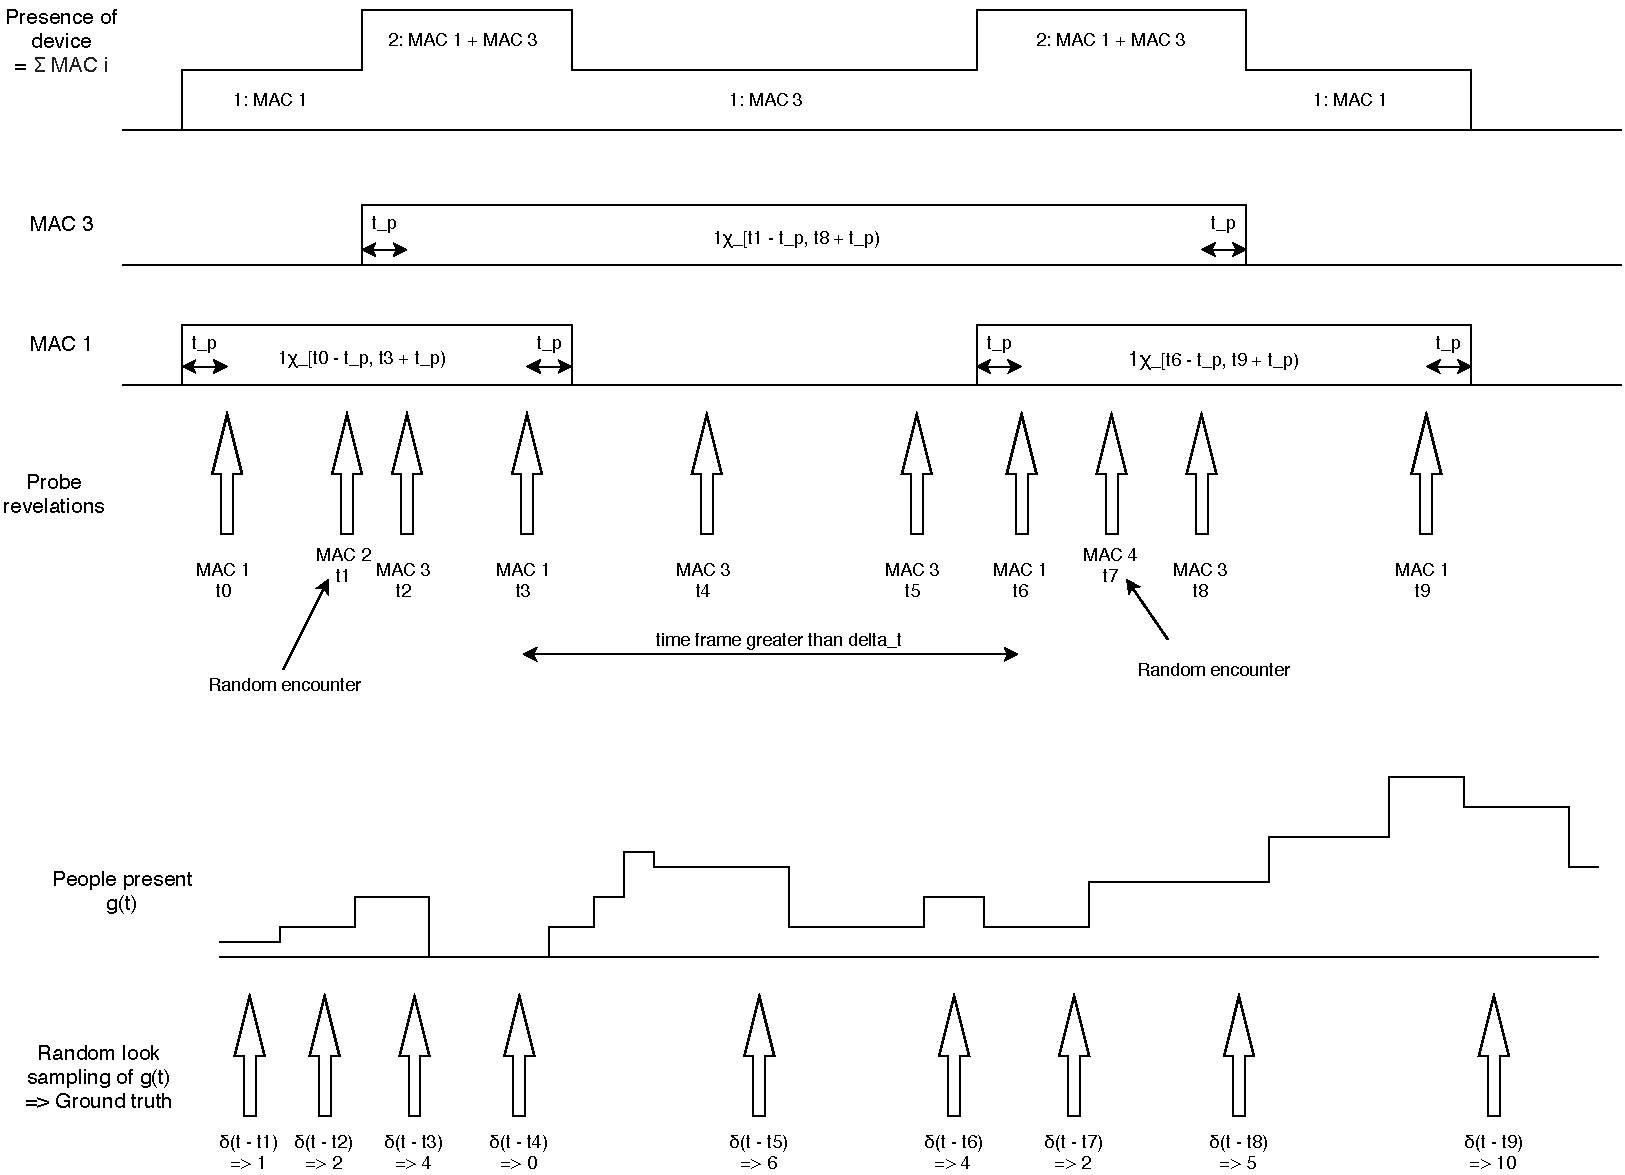
\includegraphics[width=0.9\textwidth]{images/timeprocesses} 
\caption{Illustration of the management of the different time processes.}
\label{fig:timeprocesses}
\end{figure}


\section{Evaluation of the results}
\label{sec:evalres}
\vspace{0.2 cm} 

Once the Machine Learning model is trained with the collected ground truth and the number of devices revealed at the timestamps when the ground truth is collected, the estimates of people are generated in these timestamps. We calculated the following parameters for evaluating the proposed system estimates and satisfy the KPIs (Key Performance Indicators), taking as the ground truth the number of people I manually annotated, with a random look strategy of some hours per day in different time slots:
\begin{itemize}
  \item Mean Absolute Error = mean(abs(people\_present - people\_estimated))
  \item Mean Squared Error = mean(square(people\_present - people\_estimated))
  \item For each revelation scaled\_MSE\_trend += $\Bigl(\frac{people\_present - people\_estimated}{people\_present} \Bigr)^{2}$ and in the end\\Scaled\_MSE\_trend/revelation = $\frac{scaled\_MSE\_trend}{revelation}$
  \item For each revelation scaled\_MAE\_trend += abs$\Bigl(\frac{people\_present - people\_estimated}{people\_present} \Bigr)$ and in the end\\Scaled\_MAE\_trend/revelation = $\frac{scaled\_MAE\_trend}{revelation}$
\end{itemize}

In figure~\ref{fig:testresults}, some results and useful processing information are reported.

\begin{figure}[h]
\centering 
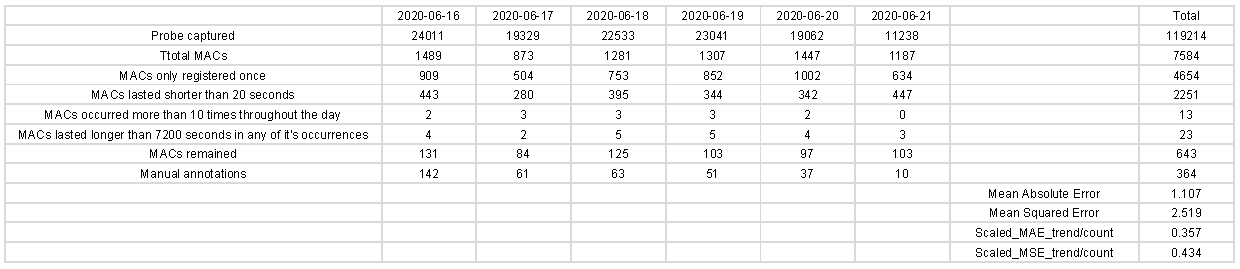
\includegraphics[width=1\textwidth]{images/testresults} 
\caption{Illustration of the results and useful processing information.}
\label{fig:testresults}
\end{figure}

% Finally, in figure~\ref{fig:comparison},~\ref{fig:differentseries},~\ref{fig:absoluteerror},~\ref{fig:errorpres},~\ref{fig:scatterplotpres},~\ref{fig:errorest},~\ref{fig:scatterplotest} there are some graphs created to show the Machine Learning results in terms of errors and comparison of the estimates between revealed devices and the ground truth.

Finally, in figure~\ref{fig:comparison},~\ref{fig:absoluteerror},~\ref{fig:errorpres},~\ref{fig:scatterplotpres},~\ref{fig:scatterplotest} there are some graphs created to show the Machine Learning results in terms of errors and comparison of the estimates between revealed devices and the ground truth.

\begin{figure}[h]
\centering 
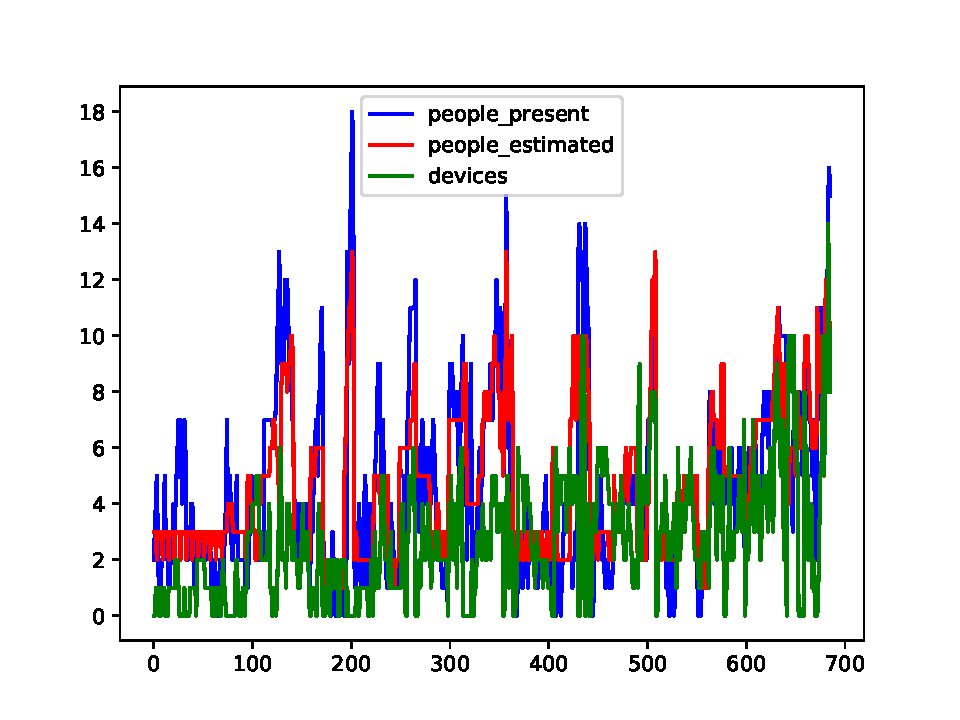
\includegraphics[width=0.8\textwidth]{images/comparison} 
\caption{Comparison between estimates, revealed devices and ground truth.}
\label{fig:comparison}
\end{figure}

% \begin{figure}[h]
% \centering 
% 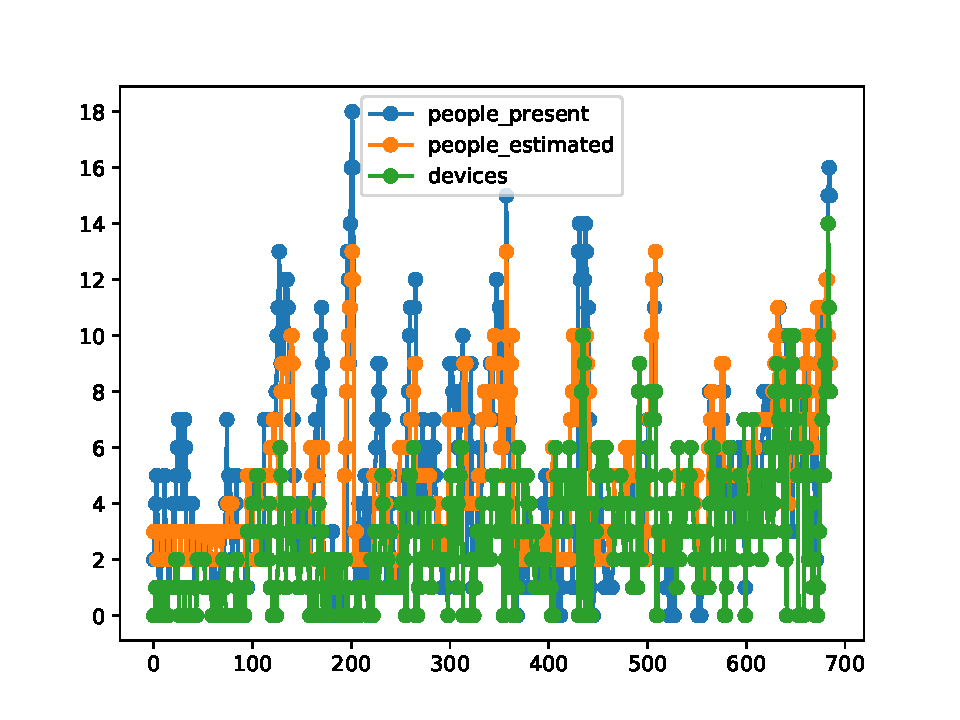
\includegraphics[width=0.8\textwidth]{images/differentseries} 
% \caption{Comparison between estimates, revealed devices and ground truth.}
% \label{fig:differentseries}
% \end{figure}

% \begin{figure}[h]
% \centering 
% 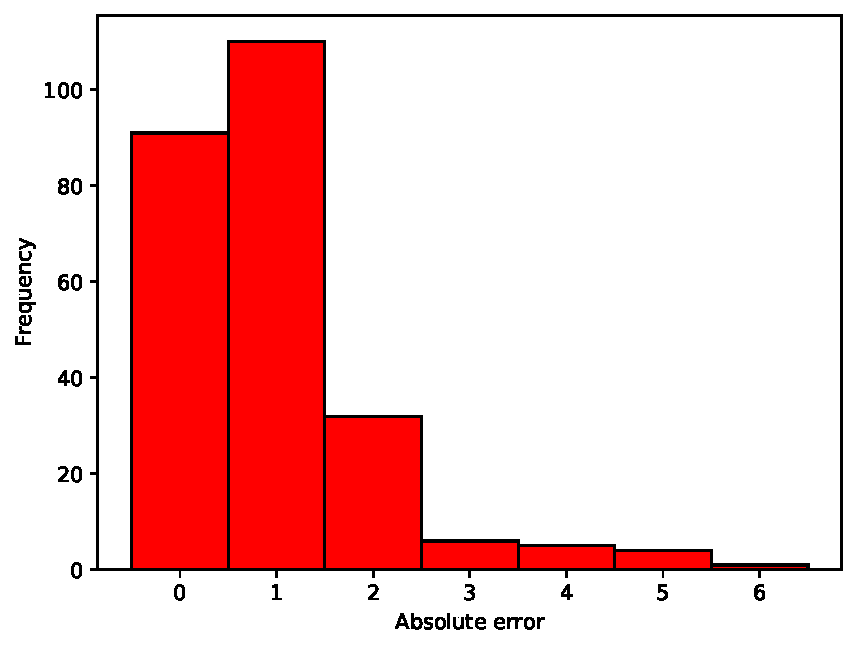
\includegraphics[width=0.8\textwidth]{images/absoluteerror} 
% \caption{Graph illustrating the distribution of the absolute error.}
% \label{fig:absoluteerror}
% \end{figure}

% \begin{figure}[h]
% \centering 
% 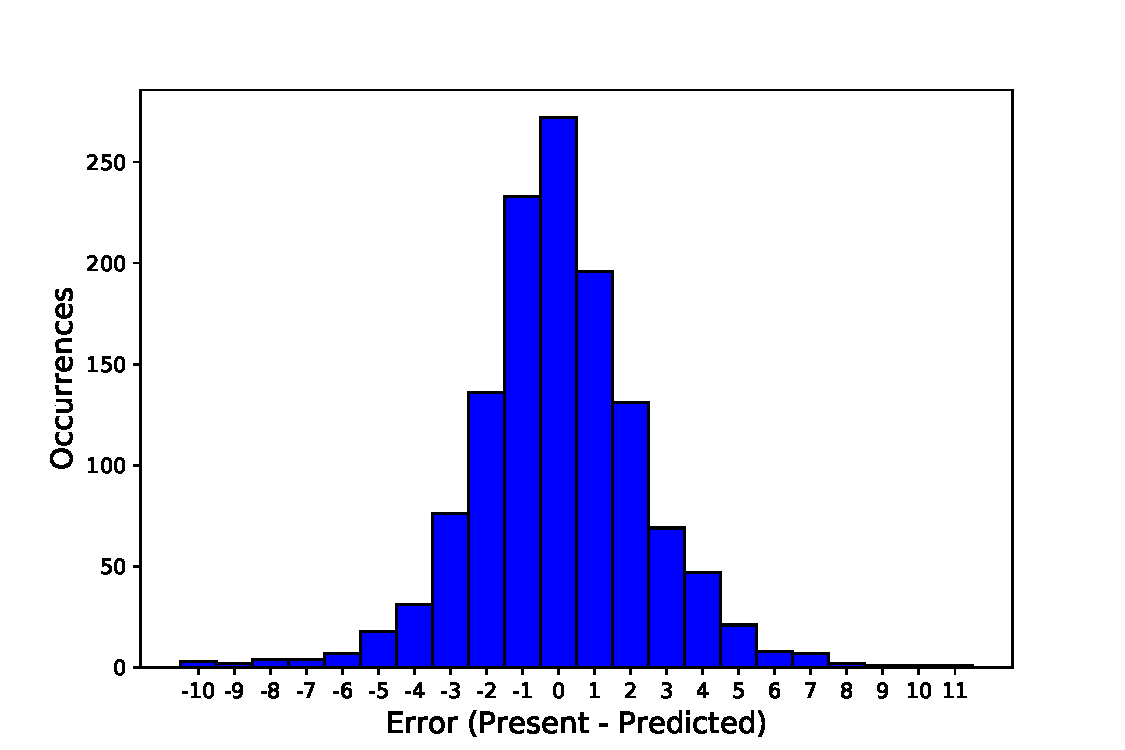
\includegraphics[width=0.8\textwidth]{images/errorpres} 
% \caption{Graph illustrating the distribution of the error.}
% \label{fig:errorpres}
% \end{figure}

\begin{figure}[h!]
\begin{minipage}[b]{8.5cm}
\centering
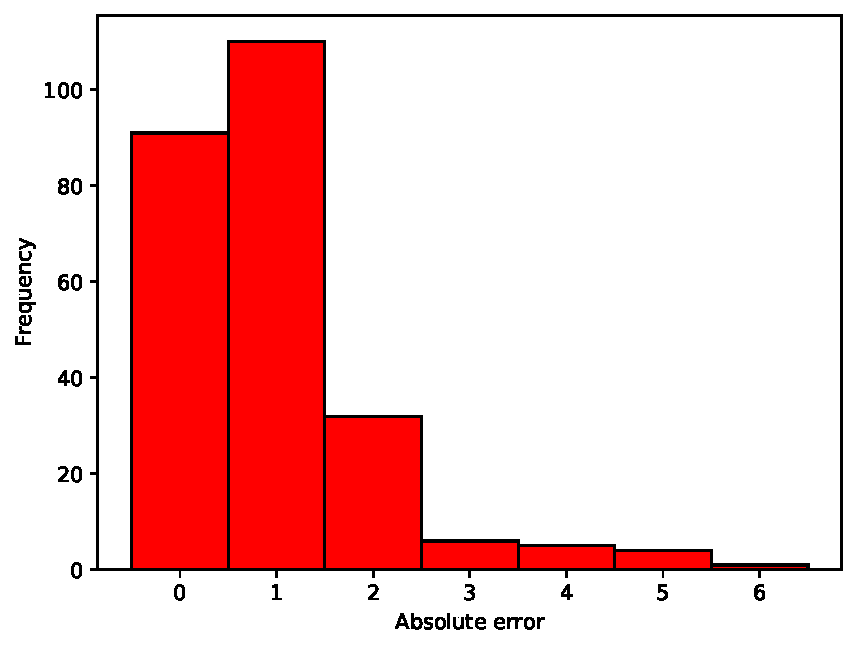
\includegraphics[width=0.85\textwidth]{images/absoluteerror}
\caption{Graph illustrating the distribution of the absolute error.}
\label{fig:absoluteerror}
\end{minipage}
\ \hspace{2mm} \hspace{3mm} \
\begin{minipage}[b]{8.5cm}
\centering
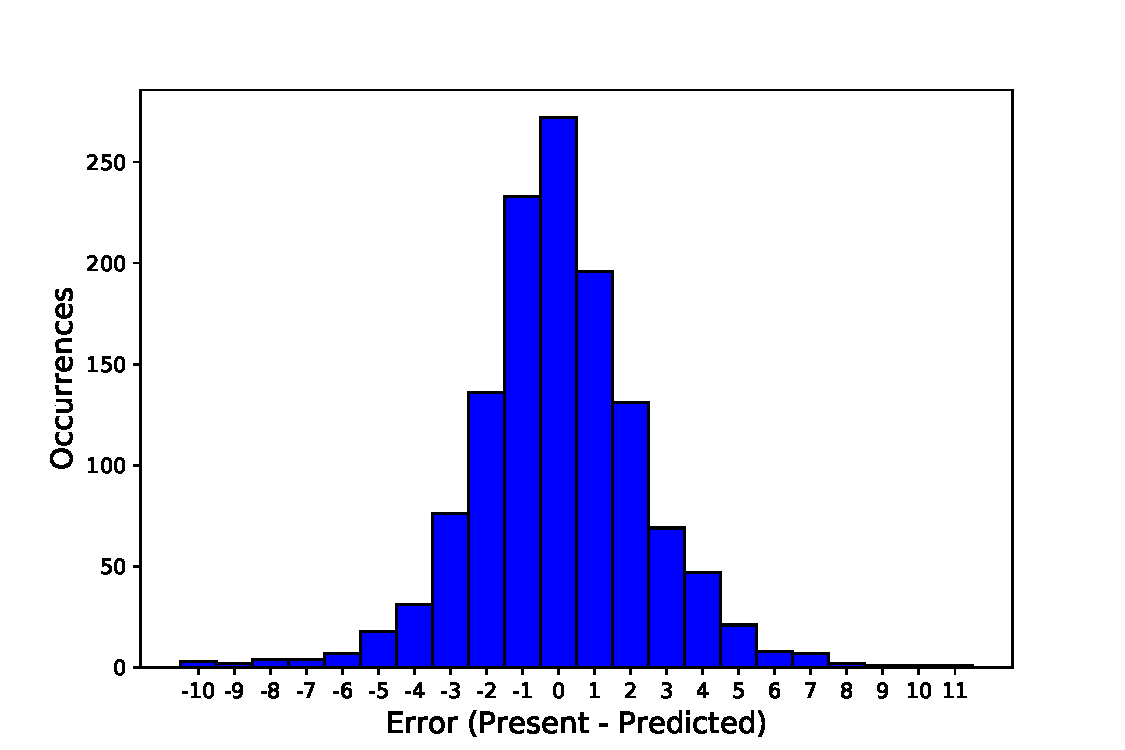
\includegraphics[width=0.85\textwidth]{images/errorpres}
\caption{Graph illustrating the distribution of the error.}
\label{fig:errorpres}
\end{minipage}
\end{figure}

% \begin{figure}[h]
% \centering 
% 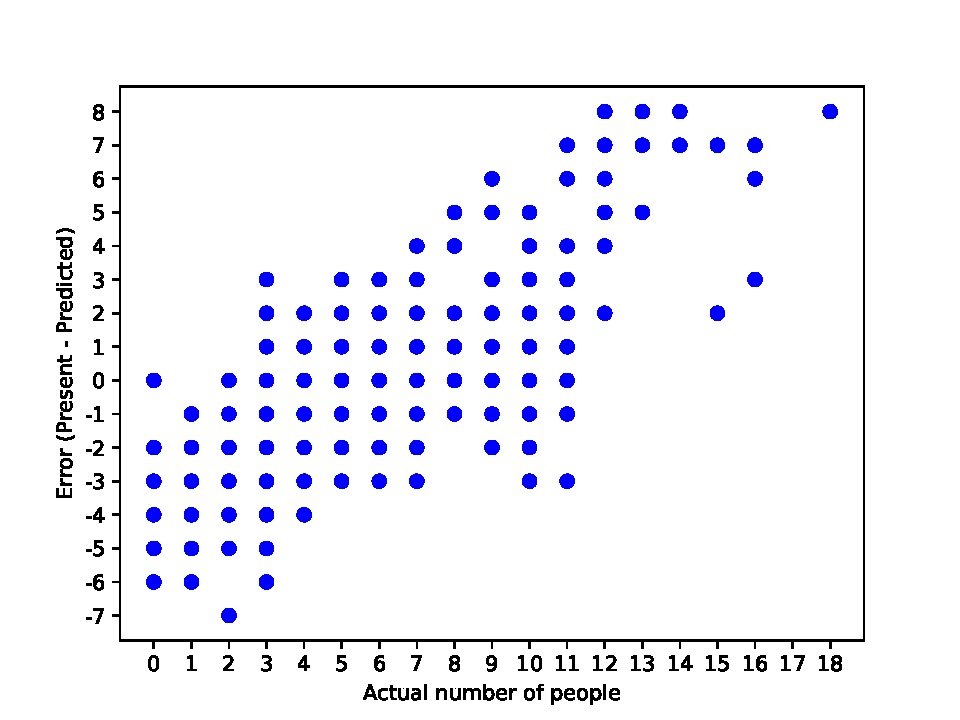
\includegraphics[width=0.8\textwidth]{images/scatterplotpres} 
% \caption{Scatter plot illustrating how the error is distributed in relation to the present number of people.}
% \label{fig:scatterplotpres}
% \end{figure}

% \begin{figure}[h]
% \centering 
% 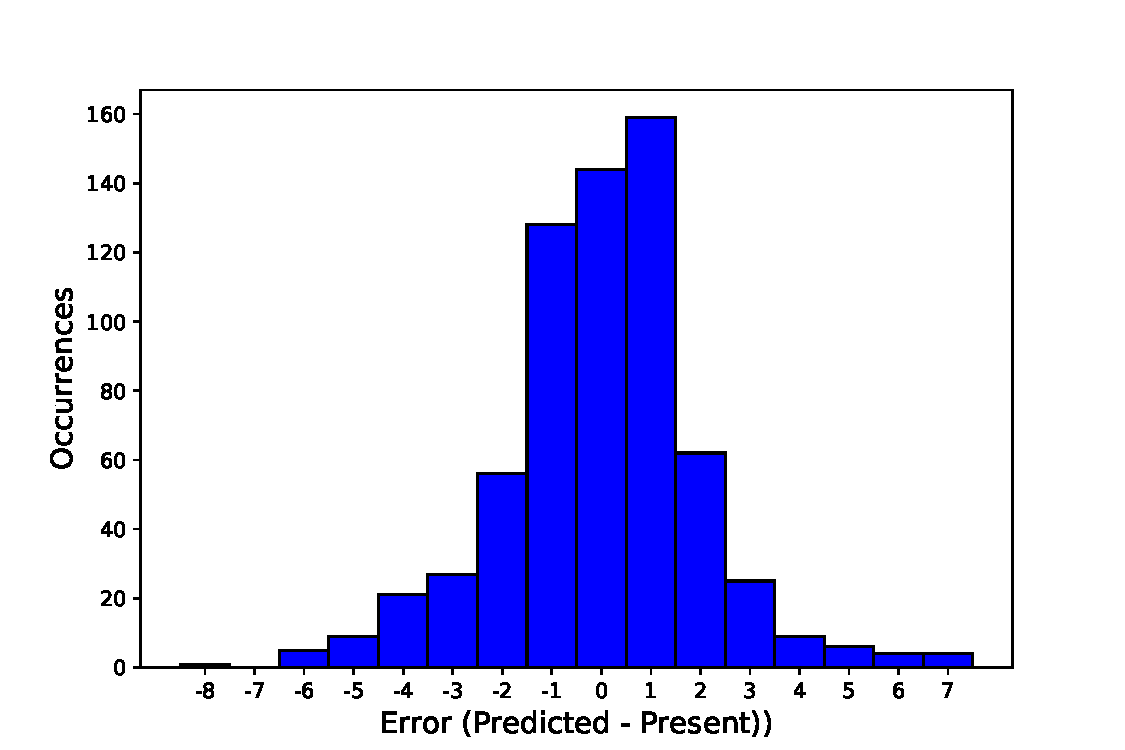
\includegraphics[width=0.8\textwidth]{images/errorest} 
% \caption{Graph illustrating the distribution of the error.}
% \label{fig:errorest}
% \end{figure}

% \begin{figure}[h]
% \centering 
% 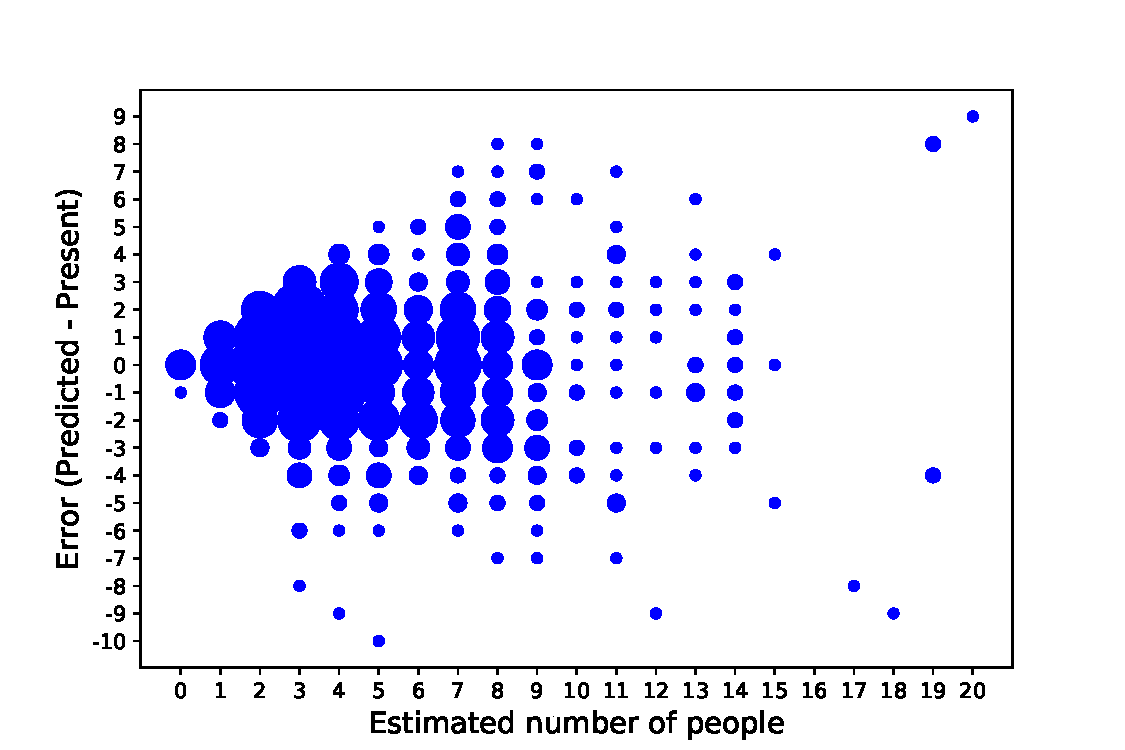
\includegraphics[width=0.8\textwidth]{images/scatterplotest} 
% \caption{Scatter plot illustrating how the error is distributed in relation to the estimated number of people.}
% \label{fig:scatterplotest}
% \end{figure}

\begin{figure}[h!]
\begin{minipage}[b]{8.5cm}
\centering
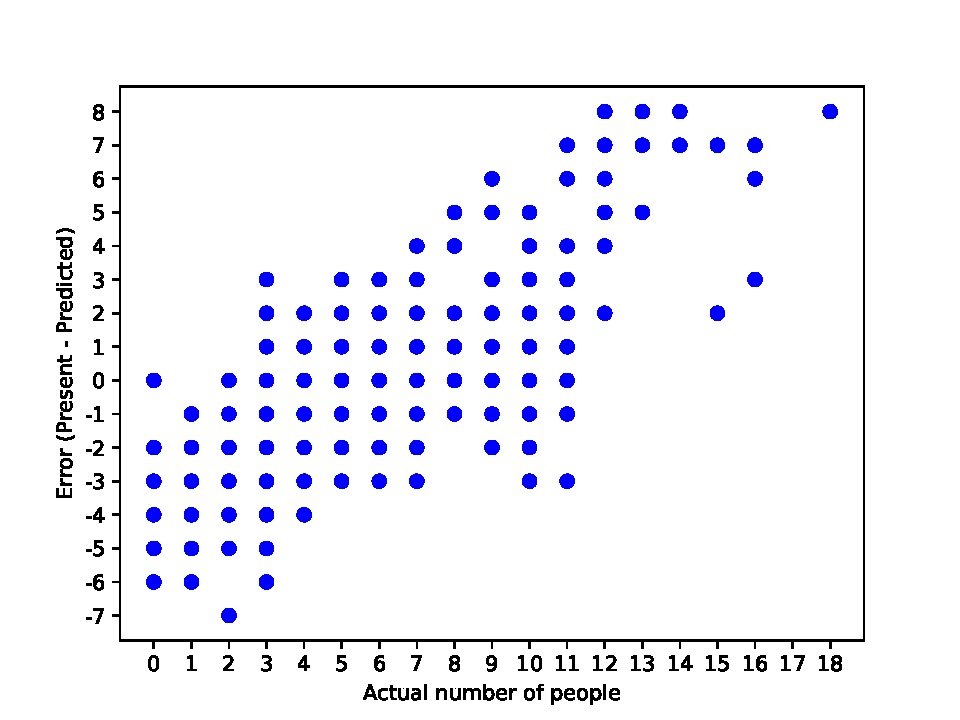
\includegraphics[width=0.85\textwidth]{images/scatterplotpres}
\caption{Scatter plot illustrating how the error is distributed in relation to the present number of people.}
\label{fig:scatterplotpres}
\end{minipage}
\ \hspace{2mm} \hspace{3mm} \
\begin{minipage}[b]{8.5cm}
\centering
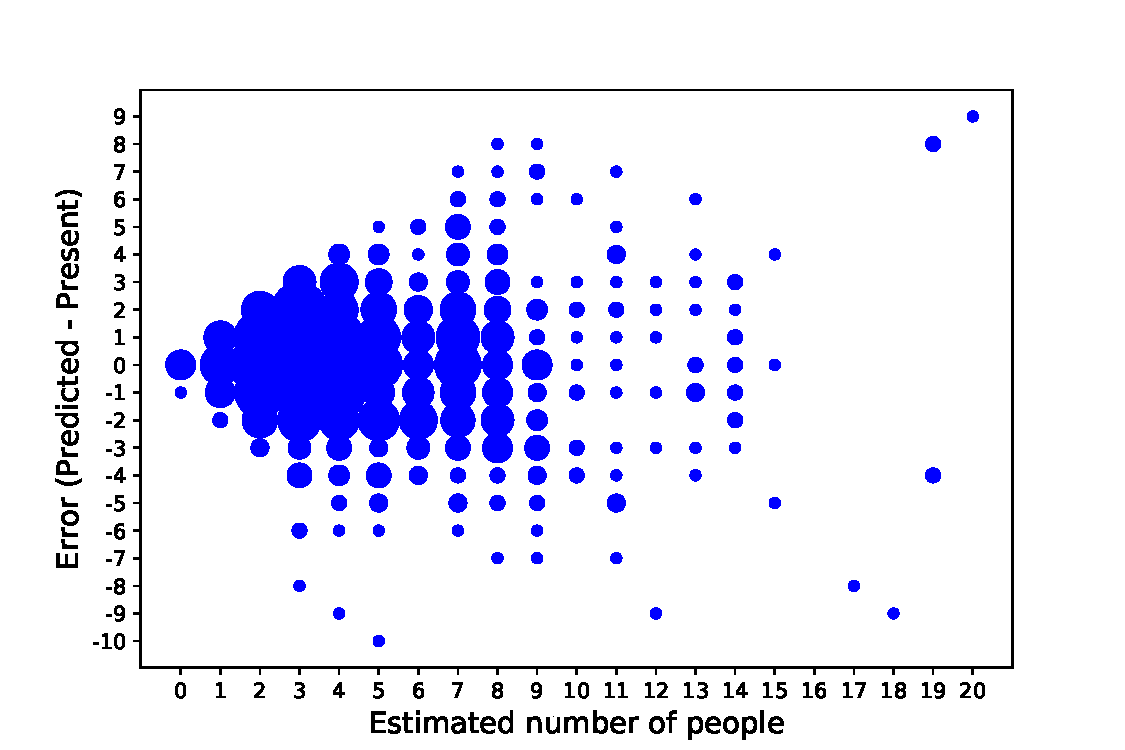
\includegraphics[width=0.85\textwidth]{images/scatterplotest}
\caption{Scatter plot illustrating how the error is distributed in relation to the estimated number of people.}
\label{fig:scatterplotest}
\end{minipage}
\end{figure}

% In figure~\ref{fig:devicespredictions}, ~\ref{fig:esteemseries} there are some graphs created to show the Machine Learning results in terms of comparison of the estimates between revealed devices on all the time series when the Wi-Fi probe request frames are revealed.

In figure~\ref{fig:devicespredictions} there is a graph created to show the Machine Learning results in terms of comparison of the estimates between revealed devices on all the time series when the Wi-Fi probe request frames are revealed.

\begin{figure}[h]
\centering 
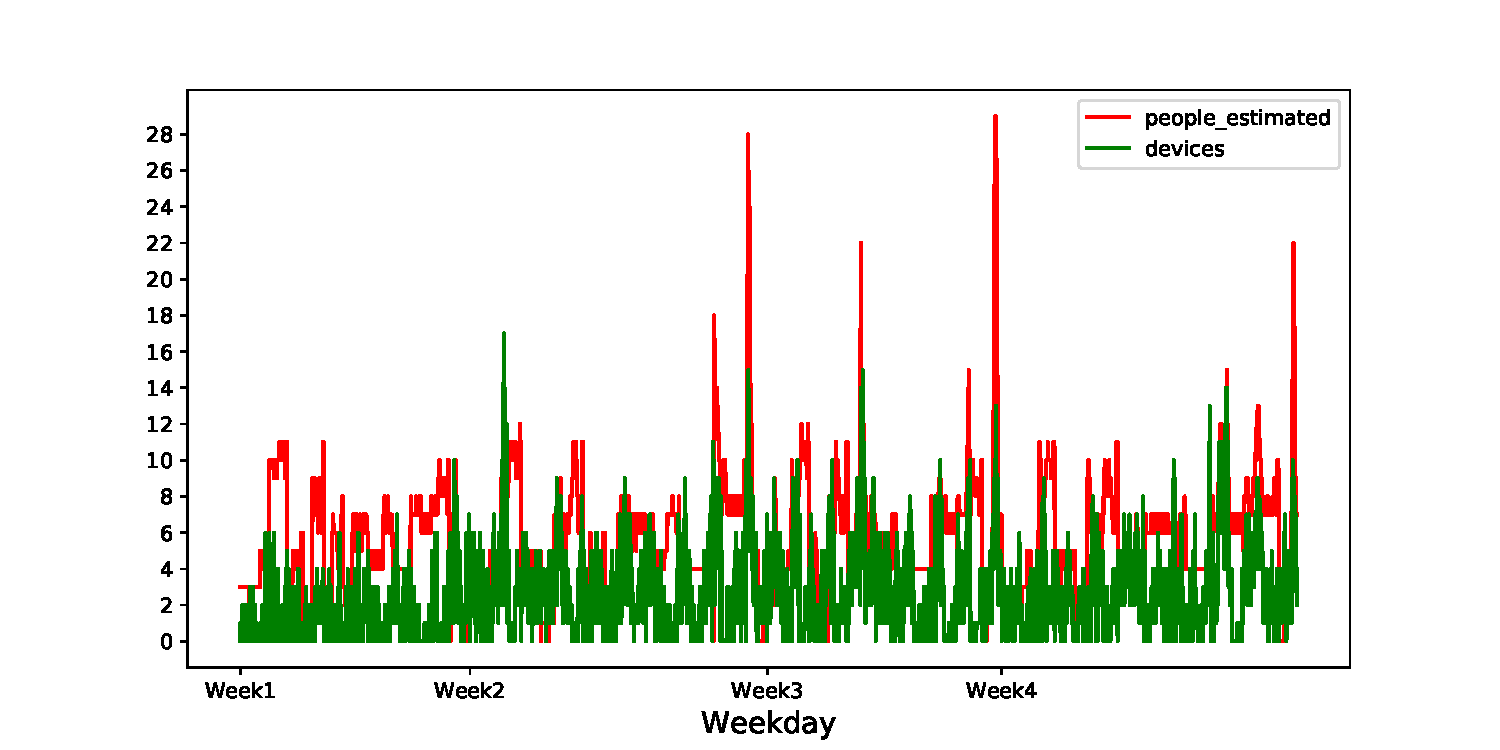
\includegraphics[width=0.8\textwidth]{images/devicespredictions} 
\caption{Comparison between estimates and revealed devices.}
\label{fig:devicespredictions}
\end{figure}

% \begin{figure}[h]
% \centering 
% 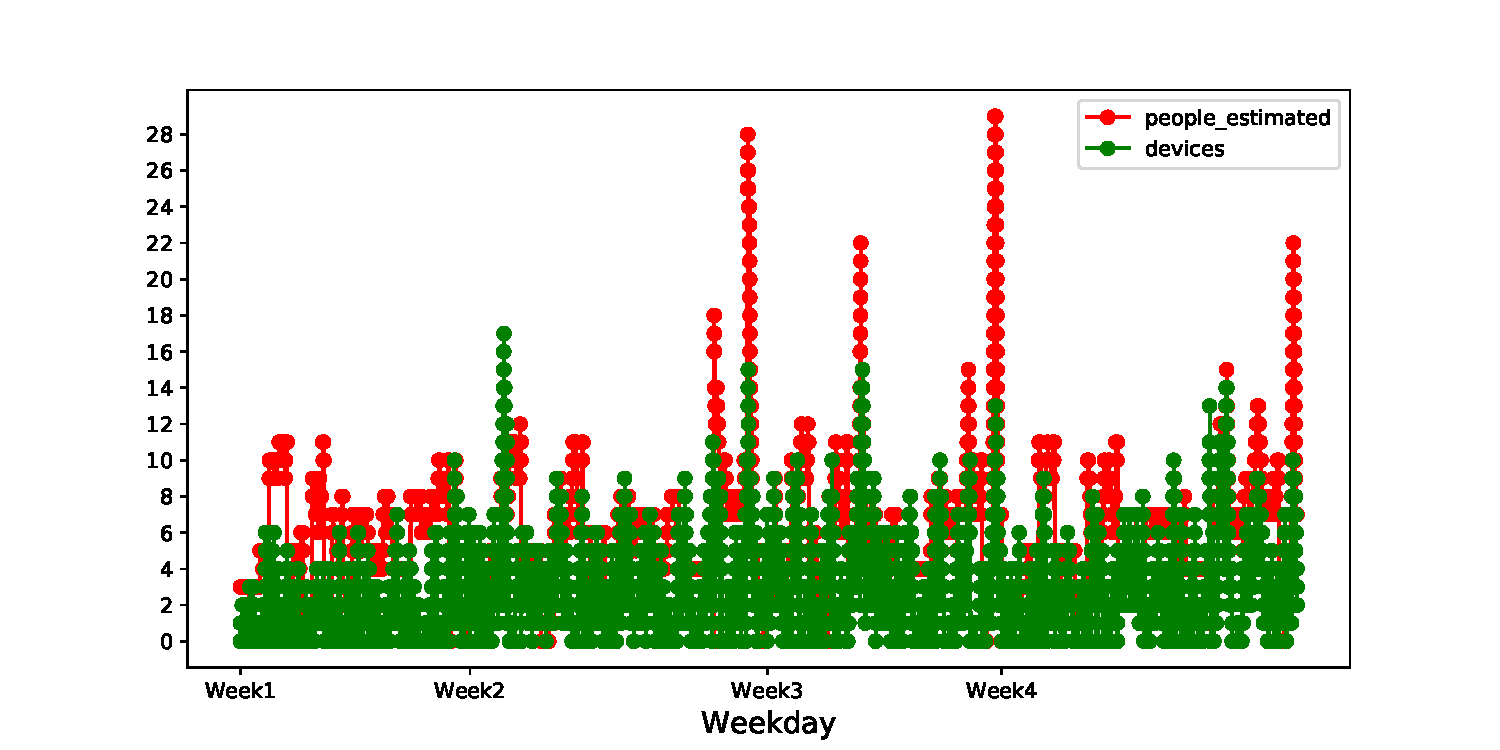
\includegraphics[width=0.8\textwidth]{images/esteemseries} 
% \caption{Comparison between estimates and revealed devices.}
% \label{fig:esteemseries}
% \end{figure}
